\section{Camera Module (jc)}
\label{sec:John_options}

A range of different camera modules were researched and considered for use in the project.

\subsection{Approach: Compact Digital Camera}
\label{sec:Compact_option}
A huge range of compact digital cameras are available for purchase and this was considered as a possible approach.

Advantages:
      \begin{itemize}
         \item High resolution of typically 5+ Megapixels.
		 \item Fully encapsulated.
		 \item High quality images possible thanks to automatic focus and zoom.
     \end{itemize}

Disadvantages:
     \begin{itemize}
        \item Difficult/impossible to communicate with: most modern digital cameras have a USB socket for downloading images off the camera but it is much rarer to be able to send the camera commands (e.g. take photo) and for those cameras where it is possible the command structure is not usually simple.
        \item Requires USB host device in order to properly communicate as only USB host devices provide power via USB and can have USB peripherals connected to them.
	\item Relatively large and heavy compared to the other approaches considered.
	\item Expensive, prices starting around \pounds 60.
     \end{itemize}

In order to communicate with a camera via USB a USB host is required. The process is usually fairly complex so driver is normally used. This is extremely difficult to implement on a device compact enough for use in this project.

\subsection{Approach: USB Camera}
\label{sec:USB_option}
Many USB webcams are available for purchase and this was considered as a possible approach.

Advantages:
      \begin{itemize}
         \item Low cost of typically around \pounds 15.
         \item High resolution of typically 1 to 3 Megapixels.
		 \item Small size of usually less than 50mm by 50mm.
		 \item Cabling included so can be easily positioned in the UAV.
     \end{itemize}

Disadvantages:
\begin{itemize}
     \item Often poorly documented: no datasheets or datasheets aimed solely at use with a computer.
     \item Difficult to communicate with: These devices are usually designed to be used with a computer so communication is usually done using a proprietary driver (a piece of software that defines how to interact with a peripheral). In order to maintain the proprietary nature of these documentation and/or source code is often not available for them.
    \item Requires USB host device in order to properly communicate as only USB host devices provide power via USB and can have USB peripherals connected to them.
	\item High resolution means longer total transfer times, including time to transfer from the camera and time spent on any compression/ manipulation.
\end{itemize}

In order to communicate with a USB camera a USB host is required, and as the process is usually fairly complex a driver is normally used. These drivers are fairly complex pieces of code and they are designed for use on computers, they are also often poorly documented so it would be extremely difficult to implement them on a device compact enough for use in this project.

\subsection{Approach: Analogue Camera}
\label{sec:Analog_option}

Camera modules with analogue composite outputs are available, usually for cctv or surveilence purposes, and were also considered as an approach.

Advantages:
\begin{itemize}
	\item Range of resolutions available.
	\item Small size: usually less than 50mm x 50mm.
	\item This is a mature market so there are plenty of options available.
\end{itemize}

Disadvantages:
     \begin{itemize}
        \item Awkward to communicate with: in order to decode the output of these devices we either need to convert from analogue to digital and then decode the signal (this type of camera usually outputs in composite or component format both of which are complex encodings, particularly when converted to digital) or put the signal through a decoder IC which are better documented but still complex, and the correct chip must be used.
        \item Require case and cabling for placement in UAV.
		\item Can be expensive at up to around \pounds 80.
		\item Often video rather than still cameras.
		\item Often black and white rather than colour.
     \end{itemize}

There are a very wide range of cameras of this type available with different features however there is a significant amount of additional complexity introduced by the requirement to decode the analogue output into something that can be understood by a microcontroller.

\subsection{Approach: Serial Camera Module}
\label{sec:Serial_option}

Some camera modules are available with UART rather than USB serial communications and these to were considered as an approach.

Advantages:
      \begin{itemize}
      	 \item Well documented: these cameras usually come with datasheets and are often designed for use with electronic projects.
		 \item Easy to communicate with as they do not require a USB host or and analogue to digital conversion, additionally most microcontrollers have a built in UART port.
         \item Range of resolutions available.
		 \item Small size: usually less than 50mm x 50mm.
		 
     \end{itemize}

Disadvantages:
     \begin{itemize}
       	\item Require case and cabling for placement in UAV.
	\item Moderately expensive at around \pounds 40.
       	\item The lack of case means that the camera is susceptible to shorts and static.
     \end{itemize}

The ability to communicate via UART combined with the good documentation should allow for control to be established fastest with this camera type.

\section{Approach Chosen: Serial Camera module (jc)}
\label{sec:John_chosen_options}

The camera type chosen was a serial camera as described in \ref{sec:Serial_option}. We chose this camera type because it was the easiest to communicate with as it did not require a USB host or any kind of analogue to digital conversion and decoding. The serial camera type also has most of the advantages of the analogue camera type but is easier to communicate with.

The particular model chosen was uCam (microCam) or the "Camera Module - Serial JPEG TTL" from the "coolcomponents" website.

\begin{figure}[H]
        \centering
        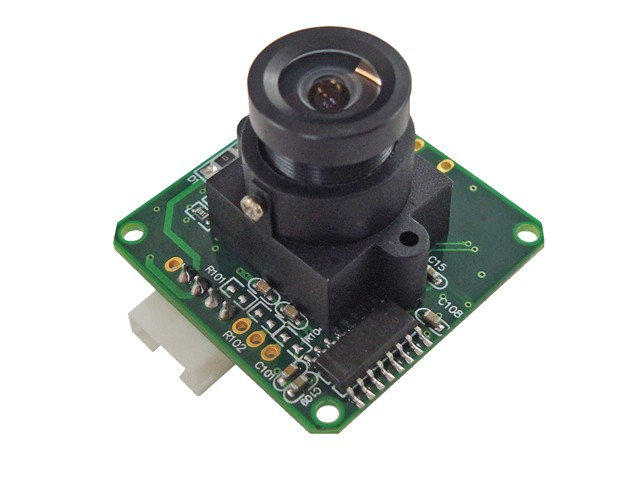
\includegraphics[width=1.00\textwidth]{figures/uCam.jpg}
        \captionof{figure}{Photo of the 4D systems uCam, sourced from \cite{ucam_datasheet}}
        \label{fig:uCam_photo}
\end{figure}

The feature set of the uCam is as follows:

	\begin{itemize}
		\item It can output images in both RAW and jpeg formats
		\item It can output RAW images at a range of resolutions:
		\begin{itemize}
			\item 80 x 60
			\item 160 x 120
			\item 320 x 240
			\item 640 x 480
			\item 128 x 128
			\item 128 x 96
		\end{itemize}
		\item It can output JPEG images at a range of resolutions:
		\begin{itemize}
			\item 80 x 64
			\item 160 x 128
			\item 320 x 240
			\item 640 x 480
		\end{itemize}
		\item It can output RAW images with a range of colour settings:
		\begin{itemize}
			\item 2bit Gray Scale
			\item 4bit Gray Scale
			\item 8bit Gray Scale
			\item 8bit Colour
			\item 12bit Colour
			\item 16bit Colour
		\end{itemize}
		\item It will auto-detect baud rates from 14400 to 115200
		\item It has selectable baud rates up to 1228800
		\item Small physical size at 32mm x 32mm
		\item Well documented
	\end{itemize}

The camera was chosen because this feature set meets the specification and also allows for additional functionality, such as setting the resolution, if the full feature set is exploited.